\begin{figure}[!b]
\begin{center}
 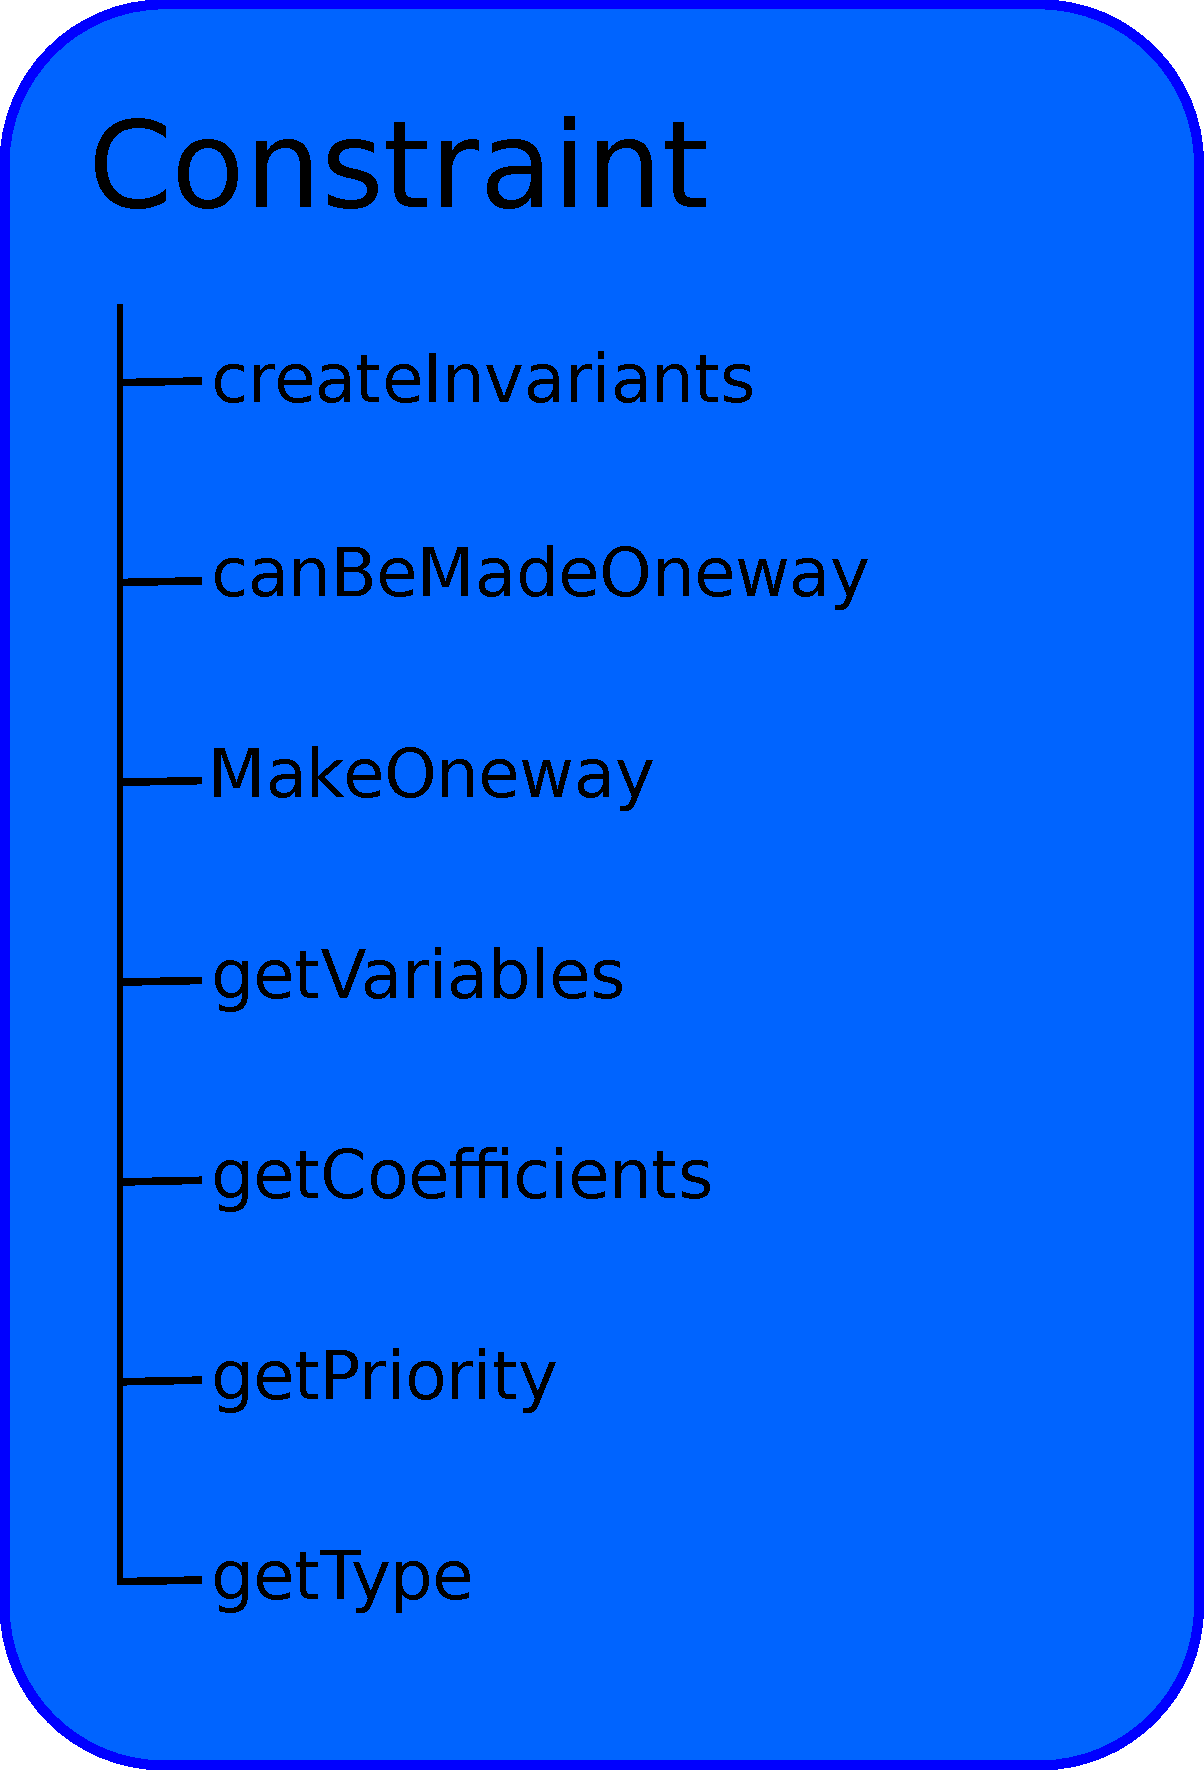
\includegraphics[width=\linewidth/2]{constraint.pdf} \caption{Important methods in Constraint 
class}\label{fig_constraint}
\end{center} 
\end{figure}
Constraints are all derived from the same class (\class{Constraint} figure \ref{fig_constraint}) that force some method 
to be implemented. All constraints needs a priority according to how important the constraint is. The priority do not 
need to be different for the constraints but it will help the local search to differentiate between infeasible  
solutions. \\ The method \method{getType} is only used if Gecode does not find an initial solution.   \\ 
A constraint is posted in the constraint programming environment and later handled by local search environment. The 
constraints are treated differently in the environments and need different parameters and methods for that. For the 
CP environment few special parameters are need such as the integer consistency level (ICL) \boste{What more?}. The LS 
environment handles constraints through invariants hence a constraint needs a method for creating the invariant(s) 
needed in LS for the specific type of constraint. \\ 
\boste{Example} \\
The Linear constraint has by definition variables, coefficients, a relation and a right hand side. When posting the 
constraint in Gecodes environment an ICL argument can be useful for guiding Gecode. In the LS environment the 
constraint is handled by creating two invariants, one for the value of the left hand side and one to determine if the 
constraint is violated. Implementation of invariants is described in next subsection and how the invariants are created 
is described in section \ref{sec_ls}. 